\documentclass{sbrt2018port}

\usepackage{flushend}

\begin{document}

\title{Um pouco da Telecomunicação no Brasil}

\author{ Acadêmico: Matheus Bazzo \\
Prof.ª: Juliana Camilo Inácio}

\maketitle

\markboth{UNIVERSIDADE DO OESTE DE SANTA CATARINA - CURSO DE ENGENHARIA DE COMPUTAÇÃO, SISTEMAS E REDES DE TELECOMUNICAÇÕES, 2018/2} {UNIVERSIDADE DO OESTE DE SANTA CATARINA - CURSO DE ENGENHARIA DE COMPUTAÇÃO, SISTEMAS E REDES DE TELECOMUNICAÇÕES, 2018/2}

\begin{resumo}
Telecomunicação é uma técnica que consiste em enviar informações a de um ponto para outro por vários meios físicos, como: cabo, sem fio, radiofrequência, satélites, entre outros, através das ondas eletromagnéticas, grande parte disso se deu inicio com a criação do telefone por Alexander Grahem Bell.
A telecomunicação abrange uma grande área de prestação de serviços, desde telefonia até TV Digital/cabo, é o setor de serviços que mais gerou lucro nos últimos anos no brasil e no mundo.
A primeira operadora de celular a chegar no brasil foi ainda na época de dom pedro II, era uma empresa estadunidense, que foi a mesma que criou a primeira conexão nacional de telefonia.
A ANATEL foi criada em 1997 junto com a lei LGT que deu inicio ao processo de privatização das empresas estatais de telecomunicações no brasil.
\end{resumo}

\begin{chave}
Operadoras, Histórico, Mercado, Telefonia móvel, Telecomunicações.
\end{chave}

\section{Introdução}

O primeiro telefone foi criado por Alexander Graham Bell em 1875, dando início a tudo o que conhecemos hoje em termos de comunicação a distancia, no brasil não demorou muito para chegar, apenas dois anos após a criação, dom pedro II trouxe para sua casa o telefone.

Em 1879 é feita a primeira conexão nacional, e por consequência nasceu a primeira empresa de telefonia brasileira a "Telephone Company of Brazil", nessa época as ligações não eram diretas, ficando a cargo das "telefonistas" fazerem a interligação manualmente por cabos.

Em 1997 a Telebras, empresa brasileira de telecomunicação é dividida, dando origem a mais doze empresas, é iniciado o processo de privatização das telecomunicações no brasil, com a lei LGT, posteriormente a isso nasce a ANATEL, empresa reguladora de telecomunicações no brasil.

Enquanto isso no mundo, em 1994 é criado pela IBM o primeiro celular com algumas funções além da conversação, como, e-mail e agenda, nasce o que conhecemos hoje por Smartphone.

\section{Mercado das Telecomunicações no Brasil}
\label{s_mercadoBrasil}
Logo após a criação da LGT, em 1997, se começou a criar um monopólio por volta de 2006, onde existiam apenas três grandes empresas de telecomunicações, CLARO, TIM e VIVO, e até hoje esse cenário não mudou muito, tendo apenas algumas mais regionais, não é atoa que o brasil tem os serviços de telefonia mais caros do mundo, segundo a UIT, União Internacional das Telecomunicações, o brasil é o 4º mais rentável do mundo em telecomunicações, mas muitas vezes não é pelo consumo e sim pelo custo.

Já o cenário de provedores de internet é mais abrangente, principalmente em questão regional, onde é mais barato e fácil vender internet fixa à população, hoje o brasil conta com 5.7 mil provedores de internet espalhados pelo país.

A telecomunicação foi o setor de serviços que mais teve receita no brasil nos últimos anos, apenas em 2016 o setor rendeu U\$38 bilhões e a estimativa para 2022 é de U\$45.76 bilhões.

Mas o setor de telecomunicações não tem apenas esses dois setores, o mesmo é divido em seis segmentos entre eles: Telefonia Fixa, Comunicação Móvel, Comunicação Multimídia, TV por Assinatura, Radiodifusão entre outros serviços, talvez o mais conhecido e utilizado é a comunicação móvel.

\subsection{Comunicação Móvel}
\label{s_segmento}

\begin{figure}[!ht]%[!htpb]
    \centering
    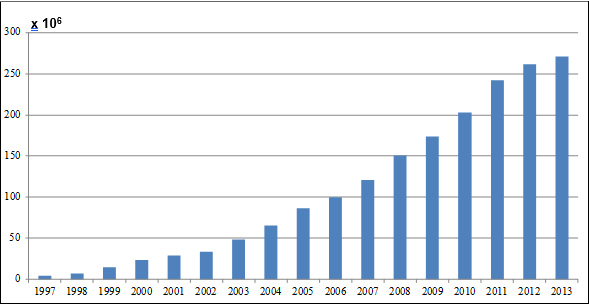
\includegraphics[width=\linewidth]{grafico.png}
    \caption{Evolução da telefonia móvel.}
    \label{f_cerd2}
\end{figure}

Comunicação móvel é o setor mais utilizado e também o mais problemático das telecomunicações no brasil, seja pelo serviço ruim, ou altas taxas, como é mostrado na figura 1, em 2003 a telefonia móvel já se igualava à telefonia fixa, que estagnou, e hoje só tende a descer, ao contrário da móvel, que já registrou 283 milhões de números, ou seja maior que a população brasileira, mas esse número não é bem distribuído entras as empresas que operam no brasil, como podemos ver na figura 2, talvez isso se de ao fato das quatro que tem maior fatia, serem nacionais e as demais regionais.

\begin{figure}[!ht]%[!htpb]
    \centering
    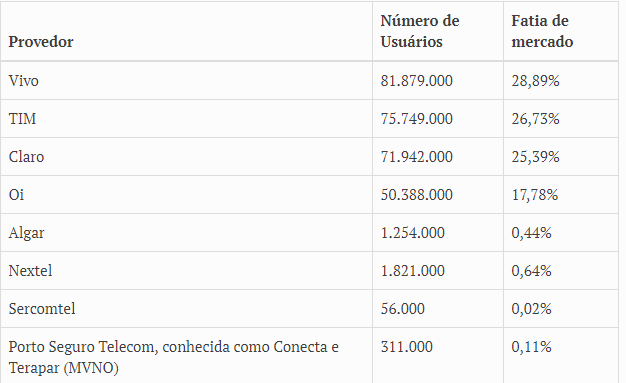
\includegraphics[width=\linewidth]{fatiamercado.png}
    \caption{Evolução da telefonia móvel.}
    \label{f_cerd2}
\end{figure}

Talvez isso se deve ao fato que os celulares já se tornaram um computador móvel, barato, em alguns casos, e de fácil acesso, o que fez esse segmento só aumentar seu valor.

Mesmo com todos os problemas, em questão de cobertura, o brasil está muito bem em comparação com o resto do globo, segundo a UIT, a cobertura 3G no brasil alcança 97\% da população e a 4G 80\%, enquanto no mundo a média de cobertura do 4G é de 64\%.

Em questão de avanço, em 2017 as operadoras de celulares no brasil já estavam testando a nova tecnologia 5G que promete ser mais rápida, ter menor latência e ser mais eficiente que as atuais tecnologias, nos estados unidos a Verizon, já está cadastrando clientes para utilizar a tecnologia 5G, mas por enquanto apenas na banda larga fixa, todos tem grandes expectativas no 5G, porque é ela quem irá dar o ponta pé inicial para a "internet das coisas" se tornarem algo viável no nosso meio.

A Nokia, empresa que fabrica os equipamentos para as operadoras no brasil, acha que a tecnologia tem grandes chances de chegar no país em 2019. Mas por enquanto devemos aguardar a ANATEL decidir as regulamentações e leiloar a faixa de 3.5GHZ que é utilizada pela tecnologia 5G, apesar disso em 2018 já foram lançados celulares que suportam esse nova tecnologia pela qualcomm.

\section{Conclusões}
\label{s_concl}

Com as informações pesquisadas foi possível notar o grande impacto que a telecomunicação tem no nosso dia-a-dia e nós as vezes nem percebemos, a falta que ela faria para nós, e também o quanto ela vem crescendo ao longos dos anos, em lucro, infraestrutura e em tecnologia.

Mas também o grande problema que ela pode se tornar se não for bem regularizada e administrada, como tivemos recentemente o caso da OI.

Como vimos no artigo a telefonia móvel tem muito a crescer ainda, e com a tecnologia 5G, isso só tende a aumentar, e esperasse que a relação operadora-cliente melhore e seja mais transparente.


\begin{thebibliography}{99}
\bibitem{hist}
Museu das Telecomunicações, [2015?].
\emph{Disponível em: <http://museudastelecomunicacoes.org.br/historia-das-telecomunicacoes>. Acesso em: nov. 2018.}

\bibitem{opd}
Observátorio do direito a comunicação, 2007.
\emph{Disponível em: <http://www.intervozes.org.br/direitoacomunicacao/?p=18913>. Acesso em: nov. 2018.}

\bibitem{mwa}
Associação brasileira de telecomunicações. telebrasil, 2017. 
\emph{Disponível em: <http://www.telebrasil.org.br/sala-de-imprensa/releases/8374-mercado-brasileiro-de-telecomunicacoes-e-dinamico-e-competitivo-diz-uit>. Acesso em: nov. 2018.}

\bibitem{tfmb}
BOECHAT,Lucas. TechinBrasil, 2015. Disponível em: <https://techinbrazil.com.br/expansao-da-telefonia-movel-no-brasil>. Acesso em: nov. 2018.

\bibitem{ing}
Bem mais seguro, [2017?].\emph{Disponível em: <https://blog.bemmaisseguro.com/internet-5g-no-brasil>. Acesso em: nov. 2018.}

\end{thebibliography}


\end{document}
